\documentclass[11pt]{scrreprt}
\usepackage[left=25mm,right=25mm,top=25mm,bottom=25mm]{geometry}
\usepackage[utf8]{inputenc}
\usepackage[ngerman]{babel}
\usepackage{float}
\usepackage{graphicx}
\usepackage{textcomp, gensymb}
\usepackage{caption}
\usepackage{xcolor}
\usepackage{url}
\usepackage{hyperref}
\usepackage{varioref}
\usepackage{mathtools}
\usepackage{amssymb}
\usepackage{siunitx}
\usepackage[version=4]{mhchem}
\usepackage{cleveref}
\usepackage{import}
\usepackage{pdfpages}
\usepackage{tikz}
\usepackage{booktabs} % Schönere Tabellen
\usepackage{pgfplots} \pgfplotsset{compat=1.16} % Plotten, Tabellen und vieles mehr

\begin{document}

\pagenumbering{gobble} % Verhindert die Seitennummerierung auf der Titelseite

%--------Deckblatt Versuchsprotokoll----------%
\import{chapters/}{Deckblatt}
%---------------------------------------------%

\pagenumbering{arabic} % Ab hier beginnt die Seitennummerierung
\setcounter{page}{1}   % mit Seitenzahl 1.

%--------Aufgabenblatt----------%
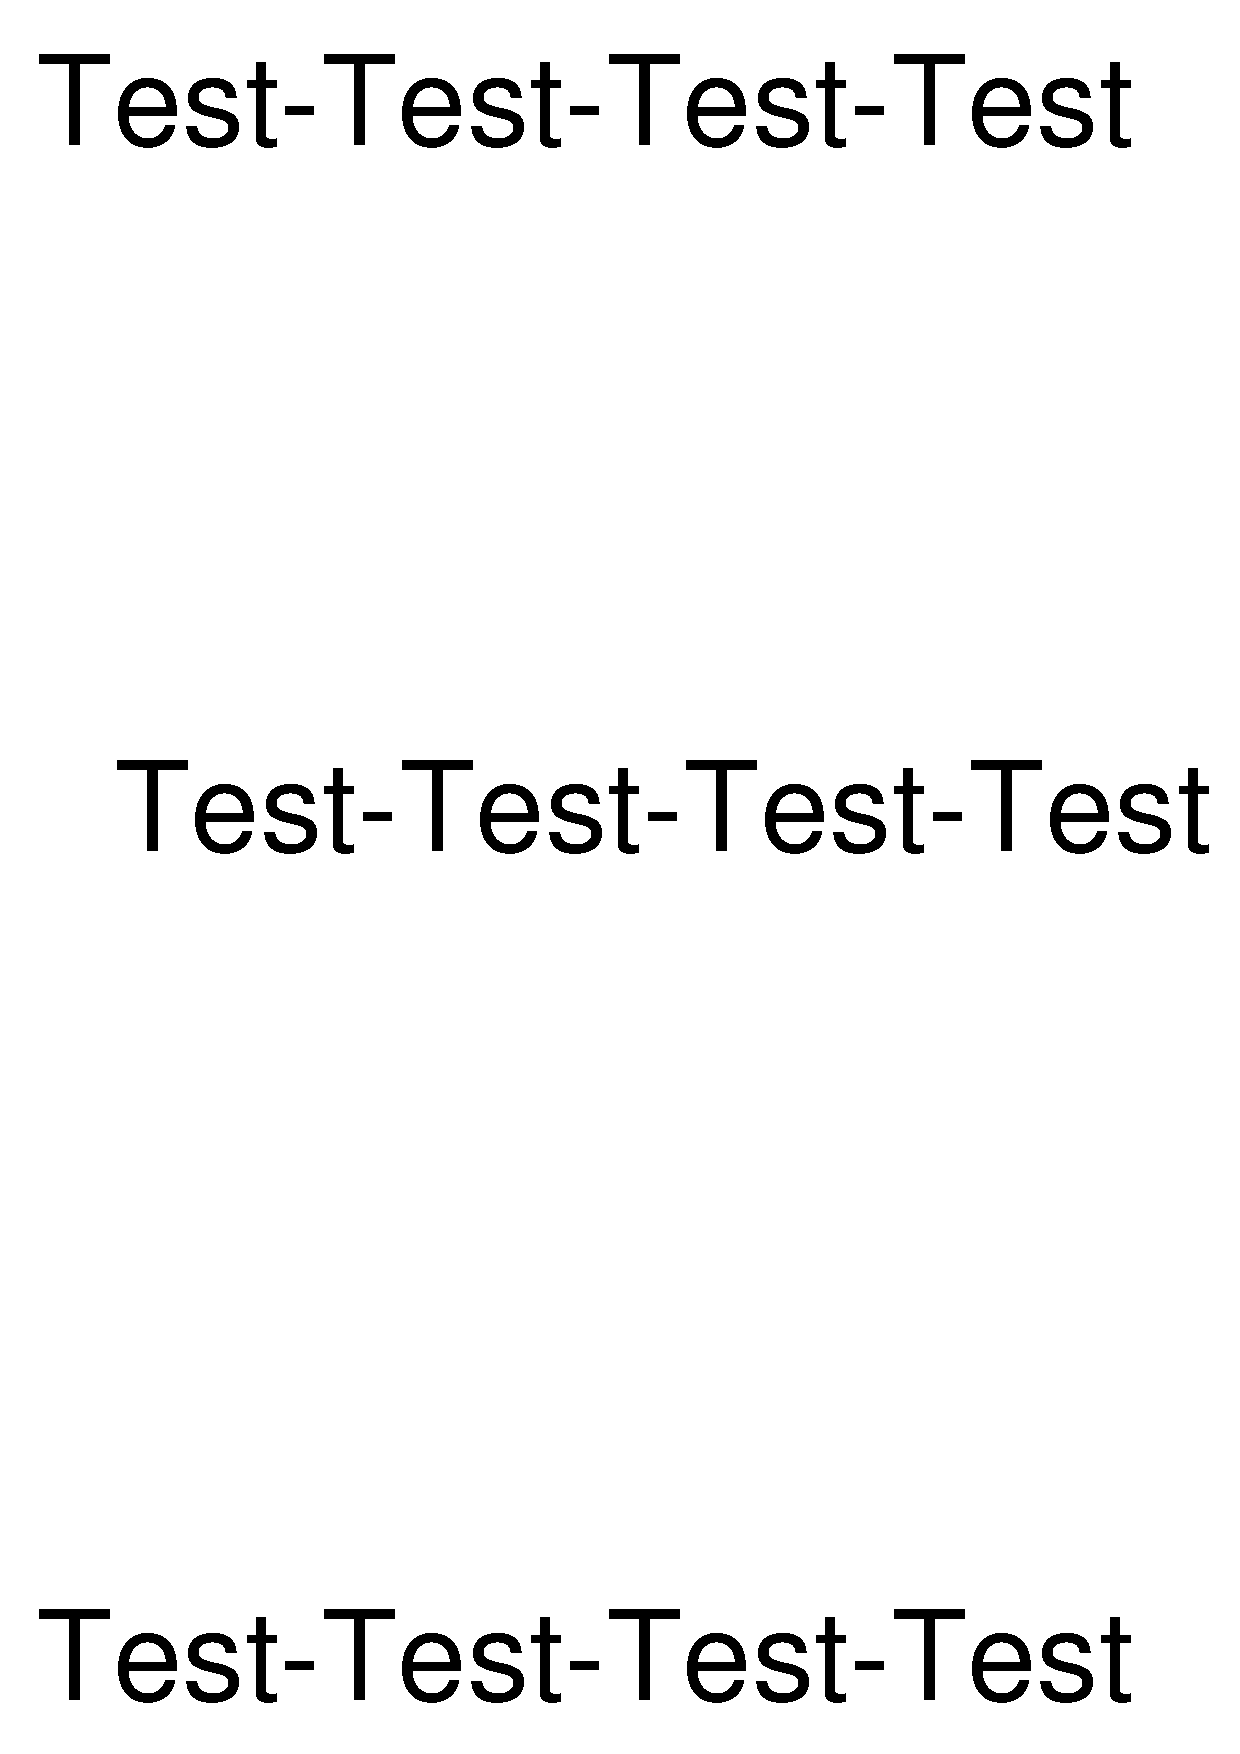
\includepdf[pages=-]{include/Aufgabenblatt.pdf} 
% Die Datei Aufgabenblatt.pdf mit dem Inhalt "Test-Test-Test-Test" muss durch das aktuelle Aufgabenblatt des Versuchs ausgetauscht werden.
%-------------------------------%

%--------Inhaltsverzeichnis und Abbildungsverzeichnis----------%
\setcounter{chapter}{-1} 
% Bei "\setcounter{section}{-1}" erhält die Einführung die Kapitelnummer "0";
% Dies kann praktisch sein, um die Kapitelnummer mit den Aufgabennummern der Versuche gleich zu halten.
% Bei "\setcounter{chapter}{0}" startet das Inhaltsverzeichnis bei "1".
\tableofcontents % Erstellt ein Inhaltsverzeichnis
%\vspace{50px}   
%\listoffigures  % Erstellt ein Abbildungsverzeichnis. Dies wird von manchen Tutor:innen gefordert.
%\vspace{50px}   
%\listoftables  % Erstellt ein Tabellenverzeichnis. Dies wird von manchen Tutor:innen gefordert.
\pagebreak
%--------------------------------------------------------------%

%--------Inhalt der Kapitel----------%
\import{chapters/}{Einführung}

\import{chapters/}{01}

\import{chapters/}{02}

\import{chapters/}{03}

\import{chapters/}{04}
%------------------------------------%

%--------Quellen----------%
\import{chapters/}{Quellen}
%-------------------------%

%--------Anhang (Messprotokoll)----------%
\chapter{Messprotokoll}
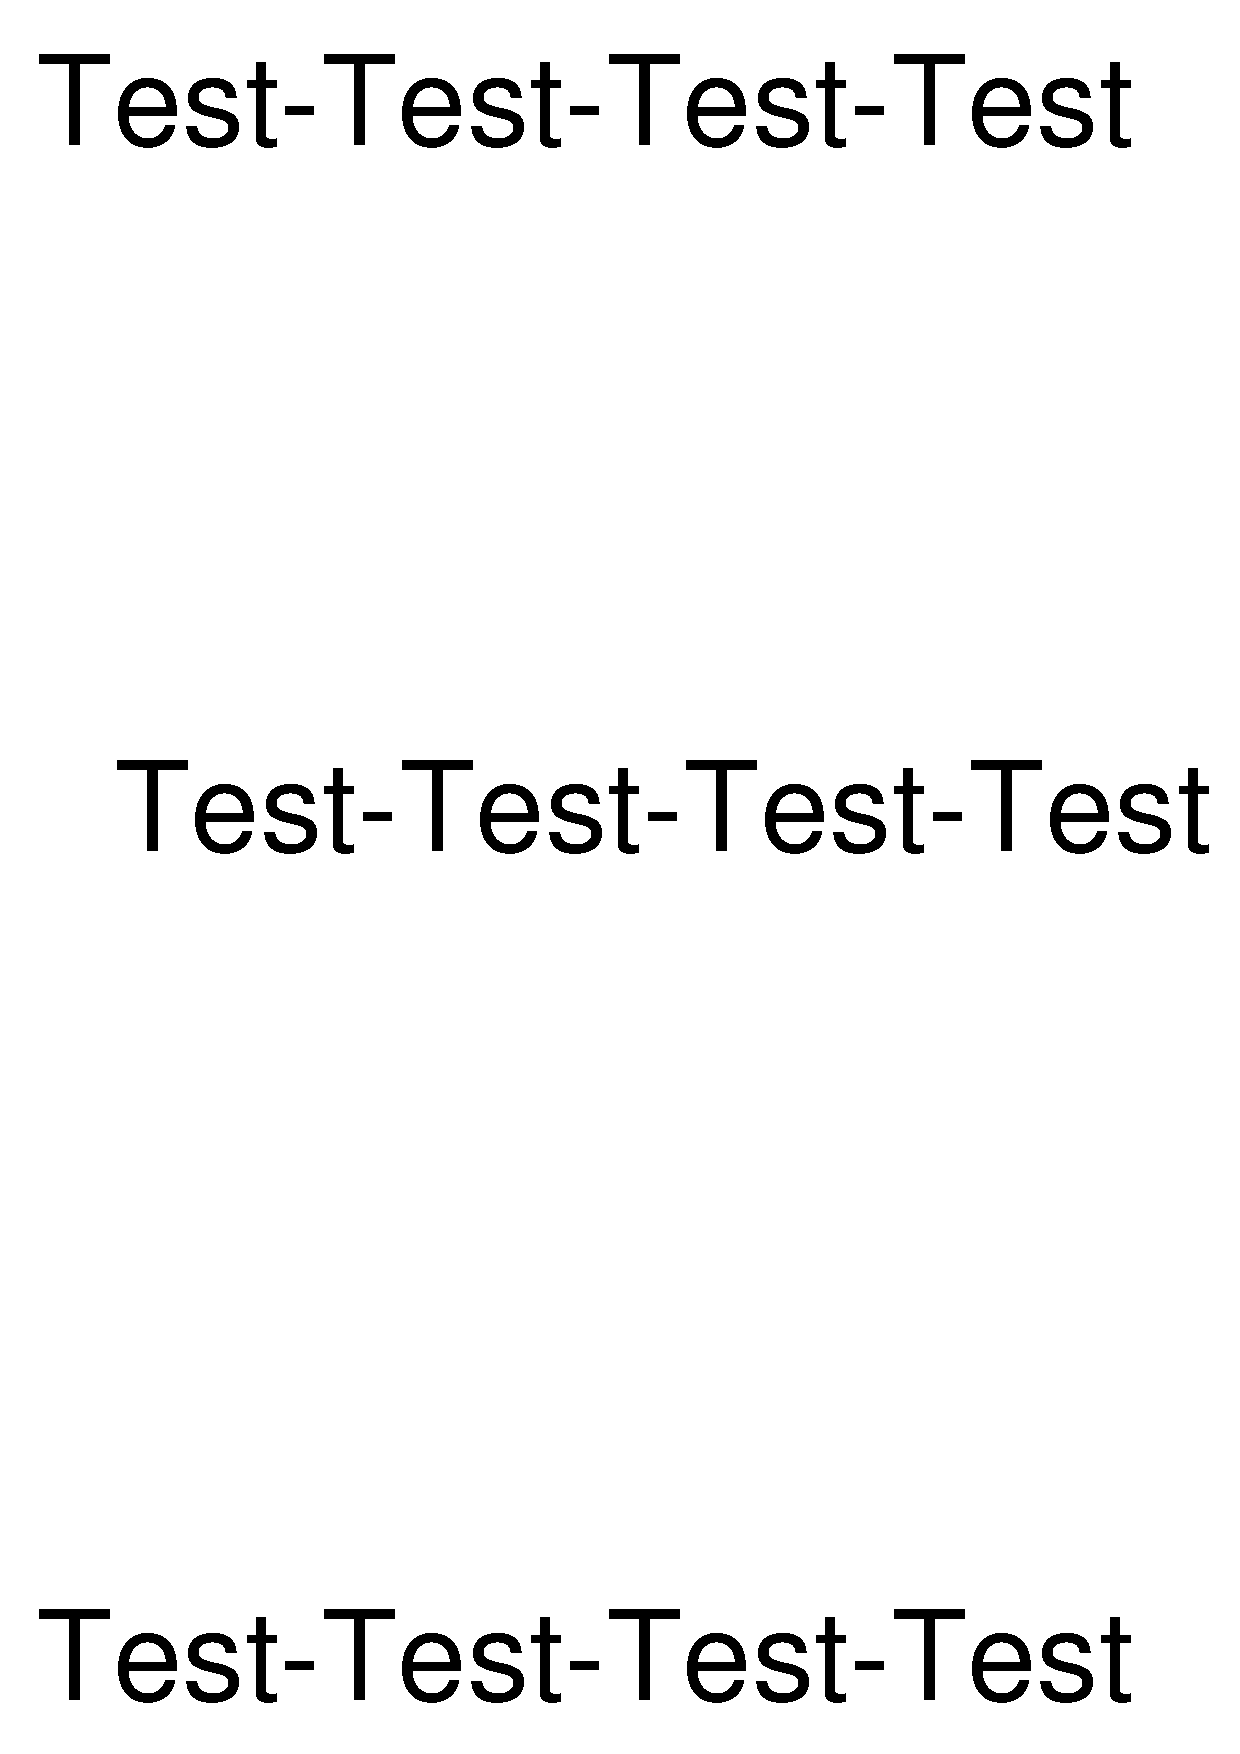
\includepdf[pages=-]{include/Messprotokoll.pdf} 
% Die Datei Messprotokoll.pdf mit dem Inhalt "Test-Test-Test-Test" muss durch das, während des Versuchs erstelltem Messprotokoll, ausgetauscht werden.
%------------------------%


\end{document}